\subsection{Background}
The most popular type of wearable in 2019 is the smartwatch \cite{best_watches}. 
Smartwatches are devices worn on one's wrist, equipped with sensors, and in some 
cases wireless communication capability for syncing data to a smartphone. They have
rich operating systems (OS), on-board processors and memory, and come in a wide range
of varieties from basic to high-end, with different specialized models in between \cite{smartwatch_arch_rit}.

% ======= TYPICAL SMARTWATCH SPECIFICATIONS =============
\subsection{Typical Specifications}
Modern smartwatches typically have similar components to computers, albeit at a much smaller scale.
They have an OS, which is most cases is proprietary to the manufacturer (i.e. watchOS for Apple);
a single- or dual-core processor ranging from 80MHz to over 1.2GHz depending on the type of watch;
up to a gigabyte of memory; battery life ranging between 18 hours to over a week; and depending on 
the watch - sensors to measure heart rate, fitness statistics, 
and atmospheric pressure \cite{smartwatch_arch_rit}.

It is simple to build a system that can accommodate all the required features of a smartwatch
using normal computing components, however the challenge with a smartwatch is weight, size, and power
consumption, as it needs to fit comfortably on the wrist, and be able to record data for at least
an entire day on a single charge. This means all components must be lightweight, and energy efficient.
According to ARM, the most necessary optimizations are using small data memories, using slower clock
speeds, and choosing a silicon process technology that will offer the lowest possible power consumption,
meaning the biggest design trade-off when designing smartwatches is between performance and 
power consumption \cite{arm_wearable}. To examine these trade-offs, two popular smartwatches will be
analyzed for the architecture decisions that went into their design and manufacturing.

% ANALYZING APPLE AND GARMIN
\subsection{Analysis of Examples}
Two popular examples of smartwatches are the Apple Watch Series 5,
and the Garmin Forerunner 235, both shown below in Figure \ref{watches:pictures}.
These devices are priced quite differently, carry different levels of functionality, and are
therefore targeted towards different market segments. Shown below in Table \ref{watch:price} are 
prices for the watches listed above \cite{apple_price} \cite{garmin_price}.

% Figure of watches
\begin{figure}[h]
    \centering
    \begin{subfigure}{.5\textwidth}
      \centering
      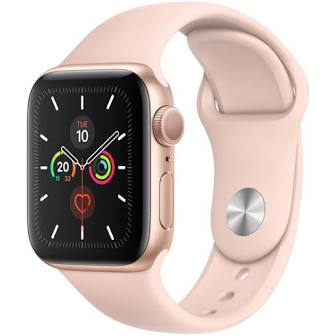
\includegraphics[width=.4\linewidth]{media/apple_pic.jpeg}
      \caption{Apple Watch Series 5 \cite{apple_price}}
      \label{fig:sub1}
    \end{subfigure}%
    \begin{subfigure}{.5\textwidth}
        \centering
        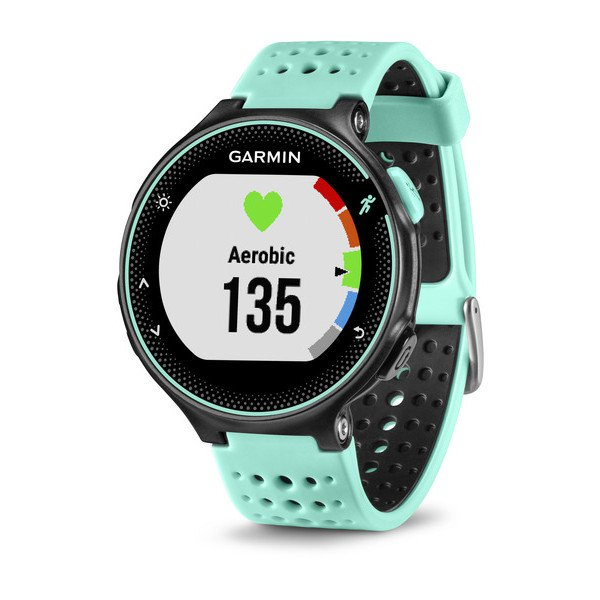
\includegraphics[width=.4\linewidth]{media/garmin_pic.jpeg}
        \caption{Garmin Forerunner 235 \cite{garmin_price}}
        \label{fig:sub3}
      \end{subfigure}
    \caption{Smartwatches discussed in this report.}
    \label{watches:pictures}
\end{figure}

% Watch prices table
\begin{table}[h]
    \centering
    \caption{Smartwatch Prices}
    \csvautotabular{data/prices.csv} 
    \label{watch:price} 
\end{table}

Clearly, these watches come at different price points, target different segments of the market, and
of course come with different architectures for accommodating the necessary features in each model. This
section will cover each of the watches shown above in greater detail.

% ========= APPLE WATCH ===============
\subsubsection{Apple Watch Series 5}
% APPLE WATCH BACKGROUND
\paragraph{Background}
The Apple Watch Series 5 is the newest iteration of smartwatch from Apple Inc., released in September
2019. Priced at \$529, clearly this is considered a higher-end smartwatch, fitting in with Apple's
other product lines (iPhone, iPad, and Mac). This watch has all-day battery life, a touch screen, 
voice call, GPS, compass, and music streaming capabilities, as well as the ability to run thousands of
apps from the Apple App Store, made specifically for the Apple Watch \cite{apple_specs}. This device
is made for Apple users, as it requires an iPhone to make use of all its features. Its operating system
is the Apple-designed watchOS.

Much of what makes the Apple Watch quite appealing is the variety of sensor technology that can track
much of your health and fitness data. This sensor technology will be discussed, along with other
computer architecture components in this section.

\paragraph{Hardware and Functionality}
An innovation brought on by the Series 5 is the always-on display, a first for Apple Watch.
An always-on display is not ideal for a device wanting low-power consumption, especially a high-resolution
screen with a high refresh rate like the one on the Apple Watch. However, this new model incorporates
a low temperature poly-silicon and oxide (LTPO) display which reduces the refresh rate of the watch's
screen from 60Hz to 1Hz, the minimum frequency for the always-on display to accurately 
display the time \cite{apple_specs}. This is a clever way to reduce power consumption by reducing frame
rate when the watch is not being used interactively. 

The processor and System in Package (SiP) at the core of the Apple Watch Series 5 is Apple's S5 chip,
shown below in Figure \ref{fig:s5chip}. This is the fifth iteration of their custom-designed 
smartwatch chip where the entire system is fabricated into a single component with a footprint
of about 40mm. This SiP includes some the sensors that come with the 
Series 5, including its GPS component and magnetometer (compass) \cite{apple_specs}.

% APPLE S5 CHIP FIGURE
\begin{figure}[h]
    \centering
    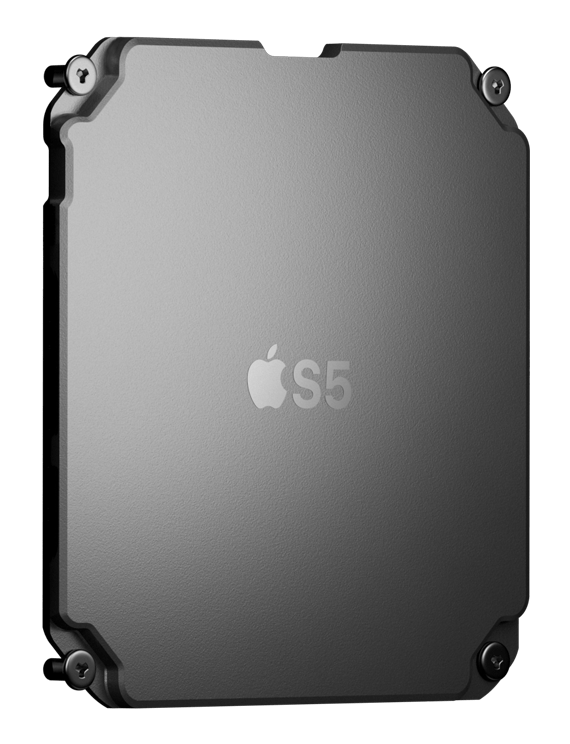
\includegraphics[width=.1\linewidth]{media/apple_s5_chip.png}
    \caption{Apple S5 Processor \cite{apple_s5_pic}}
    \label{fig:s5chip}
\end{figure}
% END APPLE S5 CHIP FIGURE

The Series 5 incorporates other sensors whose data is processed. These sensors are an electric
heart rate sensor, which constantly monitors heart rate, and can perform an electrocardiogram 
(ECG/EKG) almost as accurate as a single-lead EKG \cite{apple_health}. Data from this sensor can
be monitored and programmed to alert the wearer if there is any abnormal heart activity. The watch
also uses its microphone to monitor noise levels, and alerts the user when current noise exposure could
pose a risk for long-term hearing damage. 

Arguably the most important sensor on a smartwatch with fitness tracking capabilities is the accelerometer,
which actually tracks the motion patterns of the watch itself based on acceleration forces \cite{accel_expl}.
Data from GPS, accelerometer, heart rate monitor, and your own personal health data (height, weight, age) are
used together to give you valuable insights into your workouts. The Series 5 comes with pre-programmed
sports like cycling, running, swimming, and yoga, amongst others. In running activities, the watch
tracks and can display your calories burnt, your pace, your heart rate, your distance, cadence, and
elapsed time \cite{apple_fitness}. Having this data displayed in real time on your wrist, and available for analysis after the
run is something that makes this device so valuable, as it helps people stay motivated and quantitatively
monitor their improvements.

% =========== GARMIN =================
\subsubsection{Garmin Forerunner 235}
\paragraph{Background}
If its name wasn't obvious enough, the Garmin Forerunner 235 is first and foremost a runner's
watch.

\paragraph{Hardware}

\subsection{Smartwatch Summary}
